%\section{Block Diagrams, Linearly Invariant Systems}
\section{Lecture 4}
\subsection{System Block Diagram}
\begin{itemize}
	\item Now we'll look at how to convert an LCCDE into a block diagram. 
	\item Suppose we're given a system of the form
		\[
			\sum_{k = 0}^{N}a_k y[n - k]  = \sum_{k = 0}^{M}b_k x[n - k]
		\] 
		This implies the equation:
		\[
			y[n] = \sum_{k = 0}^{M}\frac{b_k}{a_0}x[n - k] - \sum_{k = 1}^{N}\frac{a_k}{a_0}y[n - k]
		\] 
\end{itemize}
\subsection{Linear Time Invariant (LTI), Linear Shift Invariant (LSI)}
\begin{itemize}
	\item What is an LTI system? Firstly, it's linear, so it satisfies the superposition rule: given 
		two signals \( x_1(t) \) and \( x_2(t) \), then an input of \( ax_1(t) + bx_2(t) \) will generate 
		an output of \( ay_1(t) + by_2(t) \). 
	\item An LSI is also a linear system, and given an input signal \( x(t) \) with an output 
		\( y(t) \), then we can shift
		the system \( x(t - T) \) to generate an output \( y(t - T) \), but \( y(t - T) = y(t) \). In other words, 
		the output will look like \( y(t) \), except shifted by \( T \).  
	\item As an example, the continuous LCCDE is a linear time invariant system. This is because the derivative 
		is linear: 
		\[
			\sum_{k = 0}^{M}\dv[k]{(ax_1(t) + bx_2(t)}{t} = \sum_{k = 0}^{M}b_k \dv[k]{x(t - T)}{(t - T)}
		\] 
		And then we can substitute \( u = t - T \) :
		\[
			\sum_{k = 0}^{M}b_k \dv[k]{x(u)}{u} = \sum_{k = 0}^{M}\dv[k]{y(t - T)}{(t - T)}
		\] 
	\item The same principle also holds for discrete time signals. 
	\item The most important property of an LTI system is that \textbf{the system response is fully characterized 
		by an impulse response function.}

		What this means is that if we feed the system a \( \delta(t) \) or \( \delta[n] \), it gives us an 
		impulse response function \( h(t) \) or \( h[n] \), and this gives us enough information to characterize
		the entire system.
	\item In the continuous time case, suppose we had the following:
		\begin{center}
			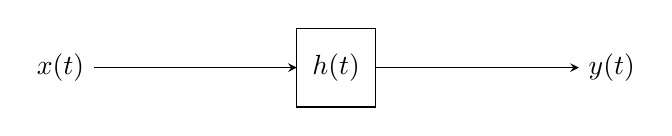
\begin{tikzpicture}
				\node (A) at (-3, 0) {\( x(t) \) };
				\node (B) at (4, 0) {\( y(t) \) };
				\draw[-stealth] (A) -- (0, 0);
				\draw (0, -0.5) rectangle node {\( h(t) \) } (1, 0.5);
				\draw[-stealth] (1, 0) -- (B);
			\end{tikzpicture}
		\end{center}
		Then, \( y(t) \), the signal generated by an arbitrary \( x(t) \) is generated by:
		\[
		y(t) = \int_{-\infty}^{\infty} x(\tau) h(t - \tau) \diff \tau 
		\] 
		In discrete time, the formula is: 
		\[
			y[n] = \sum_{k= -\infty}^{\infty} x[k] h[n - k]
		\] 
		This is called a \textit{convolution}, we will come back to this later. 
\end{itemize}
\subsubsection{Why a convolution?}
\begin{itemize}
	\item Again, consider the diagram:
	\begin{center}
			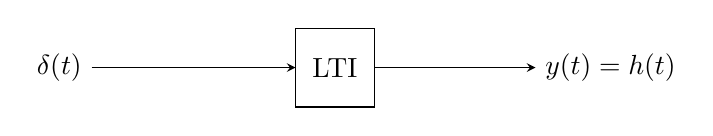
\begin{tikzpicture}
				\node (A) at (-3, 0) {\( \delta(t) \) };
				\node (B) at (4, 0) {\( y(t) = h(t)\) };
				\draw[-stealth] (A) -- (0, 0);
				\draw (0, -0.5) rectangle node {LTI } (1, 0.5);
				\draw[-stealth] (1, 0) -- (B);
			\end{tikzpicture}
		\end{center}
		If we send a signal \( \delta(t - \tau) \) into the system, then due to linear time invariance, the 
		system should output \( y(t - \tau) = h(t - \tau) \). 
	\item If we now send the signal \( x(\tau) \delta(t - \tau) \), then because \( x(\tau) \) is a constant, 
		then we invoke linearity to get that the output is  \( x(\tau) h(t - \tau) \). 
	\item Now, consider what happens when we send in the signal that is just a combination of all possible \( \tau \). 
		Each \( x(\tau) \) is a constant, so the output signal is of the form
		\[
		\int_{-\infty}^{\infty} x(\tau) \delta(t - \tau) \mapsto \int_{-\infty}^{\infty} x(\tau) h(t - \tau) 
		\diff \tau
		\] 
		But now notice that this signal can also be written as:
		\[
		\int_{-\infty}^{\infty} x(\tau) \delta(t - \tau) \diff \tau = x(t)
		\] 
		And so if we're sending in a signal \( x(t) \), then the output should be \( y(t) \)! Thus, we've proven that
		the impulse response is all we need in order to characterize \( y(t) \).
	\item For future reference, a convolution, denoted by \( x(t) * h(t) \), is defined as: 
		\[
		x(t) * h(t) = \int_{-\infty}^{\infty} x(\tau) h(t - \tau) \diff  \tau = \int_{-\infty}^{\infty} x(t - \tau)
		h(\tau) \diff \tau
		\] 
		this last equality shows that convolution is a commutative operation. 
\end{itemize}
\subsubsection{Impulse Response of 1st order LCCDE}
\begin{itemize}
	\item Recall the step response to LCCDE:
		\[
			\dv{y(t)}{t} + ay(t) = bx(t) = bu(t) \implies y_{\text{step}}(t) = 
			\left( \frac{b}{a}( 1 - e^{-at}) \right) u(t)
		\] 
	\item Given an impulse, which in this case can be written as: 
		\[
		\delta(t) = \lim_{\epsilon \to 0}\frac{u(t) - u(t - \epsilon)}{\epsilon}
		\] 
		This implies that the response \( h(t) \) is given by: 
		\[
		h(t) = \lim_{\epsilon \to 0 }\frac{y_{\text{step}}(t) - y_{\text{step}}(t - \epsilon)}{\epsilon} 
		= \lim_{\epsilon \to 0}
		\frac{\frac{b}{a}\left( e^{-a(t - \epsilon)}u(t - \epsilon) - e^{-at}u(t) \right) }{\epsilon}
		= be^{-at}u(t)
		\] 
		(verify this at home, the simplification makes use of the fact that \( e^{a\epsilon} \approx 
		1 + a\epsilon + a^2 \frac{\epsilon^2}{2} + \cdots\), but the higher order terms die).
\end{itemize}
\subsection{Harmonic Response of an LTI system}
\begin{itemize}
	\item The response of an LTI system to a complex signal \( x(t) = Ae^{j \omega t} \) is always going to be another 
		complex exponential signal \( y(t) = H(\omega) Ae^{j \omega t} \)
	\item Given the input signal \( x(t) = Ae^{j \omega t} \), we can write:
		\begin{align*}
			y(t) &= \int_{-\infty}^{\infty} x(\tau) h(t - \tau) \diff \tau\\
				 &= \int_{-\infty}^{\infty} Ae^{j \omega t}
			h(t - \tau) \diff \tau \\
				 &= \int_{-\infty}^{\infty} Ae^{j \omega (t - \tau')}h(\tau') \diff \tau'\\
				 &= Ae^{j \omega t}\underbrace{\int_{-\infty}^{\infty} e^{-j \omega \tau'}h(\tau') \diff \tau'}_{
				 H(\omega)}\\
				 &= H(\omega) Ae^{j \omega t} 
		\end{align*} 
	\item By definition:
		\[
		H(\omega) \equiv \int_{-\infty}^{\infty} e^{-j \omega \tau'}h(\tau') \diff \tau' \ \ 
		H(f) \equiv \int_{-\infty}^{\infty} e^{-j 2 \pi ft}h(t) \diff t 
		\] 
		You'll recognize \( H(\omega) \): it's the Fourier transform equation.
		
		\question{When given an harmonic input, and we're asked to measure it, are we measuring the real part 
		of the signal?}
\end{itemize}
\subsubsection{Example: Frequency response of an RC Circuit}
\begin{itemize}
	\item Given the following circuit:
		% insert circuitkkz
	\item The impulse response is given by the differential equation:
		\[
			\dv{y(t)}{t} + \frac{1}{RC}y(t) = \frac{1}{RC}x(t)
		\] 
		This is a first order LCCDE, so therefore the impulse response \( h(t) \) is given by 
		\( h(t) = be^{-at}u(t) \). 
	\item For the frequency response, we have a function of the form \( x(t) = e^{j \omega t} \), 
		which we know has an output signal of the form \( y(t) = H(\omega) e^{j \omega t} \). So all that remains
		now is to find \( H(\omega) \) :
		\begin{align*}
			y(t) &= e^{j \omega t }\int_{-\infty}^{\infty} e^{-j \omega t}h(\tau) \diff  \tau \\
			&= e^{j \omega t}\int_{-\infty}^{\infty} be^{-a\tau}u(\tau) e^{-j \omega \tau}\diff \tau  \\
			&= be^{j \omega t}\int_{0}^{\infty} e^{-a \tau}e^{-j \omega \tau}\diff \tau  \\
			&= \left( \left.-\frac{1}{a + j \omega}e^{-a \tau}e^{-j \omega t}\right|_0^{\infty}\right)
				be^{j \omega t} \\
				&= \frac{b}{a + j \omega}e^{j \omega t} 
		\end{align*}
		Now, if we impose that \( a = b = \frac{1}{RC} \), then we get the equation: 
		\[
		\frac{\frac{1}{j c \omega}}{\frac{1}{j c \omega} + R}e^{ j \omega t}
		\] 
		Now, \( \frac{1}{jc\omega} \) is the impedance of a capacitor, and this overall equation takes the form of a 
		voltage divider for a circuit with known impedance: 
		\[
		y(t) = \frac{z(\omega)}{z(\omega) + R}e^{j \omega t}
		\] 
\end{itemize}
\subsection{Sinusoidal Input} 
\begin{itemize}
	\item With the harmonic response tools, we can now evaluate the system response when given a sinusoidal 
		input, since we know that 
		\[
		\cos(\omega t) = \frac{e^{ j \omega t} + e^{- j \omega t}}{2}
		\] 
		\question{Does the same work with sine, where there's a complex number is in the denominator?} 
\end{itemize}
\subsection{LTI systems in Parallel and Series}
\begin{itemize}
	\item For a basic system with a single input and output, 
		we've already discussed that \( y(t) = x(t) * h(t) \). Now, what if we connect these systems in 
		parallel?
		\begin{center}
			\begin{tikzpicture}
				\node (A) at (-3, 0) {\( x(t) \) };
				\node (B) at (4, 0) {\( y(t) \) };
				\node (C) at (1.5, 0) {+};
				\draw[-stealth] (A) -- (-0.5, 0) -- (-0.5, 1) -- (0, 1);
				\draw (0, 0.5) rectangle node {\( h_1(t) \) } (1, 1.5);
				\draw[-stealth] (-0.5, 0) -- (-0.5, -1) -- (0, -1);
				\draw (0, -0.5) rectangle node {\( h_2(t) \) } (1, -1.5);
				\draw[-stealth] (1, 1) -- (1.5, 1) -- (C);
				\draw (C) circle (0.2cm);
				\draw[-stealth] (C) -- (B);
				\draw[-stealth] (1, -1) -- (1.5, -1) -- (C);
			\end{tikzpicture}
		\end{center}
		then, the result \( y(t) \) is given by \( y(t) = x(t) * h_1(t) + x(t) * h_2(t) = x(t) * 
		(h_1(t) + h_2(t))\).
	\item If we connect them in series: 
		\begin{center}
			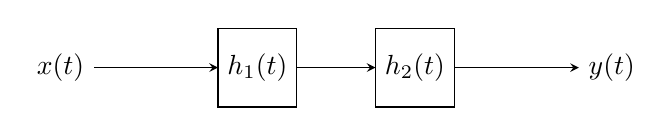
\begin{tikzpicture}
				\node (A) at (-3, 0) {\( x(t) \) };
				\node (B) at (4, 0) {\( y(t) \) };
				\draw[-stealth] (A) -- (-1, 0);
				\draw (-1, -0.5) rectangle node {\( h_1(t) \) } (0, 0.5);
				\draw[-stealth] (0, 0) -- (1, 0);
				\draw (1, -0.5) rectangle node { \( h_2(t) \) } (2, 0.5);
				\draw[-stealth] (2, 0) -- (B);
			\end{tikzpicture}
		\end{center}
		then	
\end{itemize}
